% !TEX encoding = UTF-8
% !TEX TS-program = pdflatex
% !TEX root = ../tesi.tex

%**************************************************************
\chapter{Introduzione}
\label{cap:introduzione}
%**************************************************************

% Introduzione al contesto applicativo.\\

% \noindent Esempio di utilizzo di un termine nel glossario \\
% \gls{api}. \\

% \noindent Esempio di citazione in linea \\
% \cite{site:agile-manifesto}. \\

% \noindent Esempio di citazione nel pie' di pagina \\
% citazione\footcite{womak:lean-thinking} \\

%**************************************************************
\section{Il progetto}
%Descrizione dell'azienda.
Finantix è un'azienda di informatica che vende prodotti software.
Il suo prodotto principale è suddiviso in moduli.
Ognuno di questi moduli prevede una propria documentazione delle API Java (un archivio zip contente documentazione in formato Javadoc) e la documentazione della API RESTful (un archivio zip contenente documentazione in formato Open API).
Questa documentazione viene manualmente caricata sulla piattaforma Confluence, ove cui è consultata dagli sviluppatori dell'azienda.

%Introduzione all'idea dello stage.
Il plugin Maven nasce dalla necessità di automatizzare la pubblicazione di questa documentazione su Confluence, in modo da semplificare e velocizzare notevolmente questo processo.
Infatti, una volta configurato correttamente il plugin in tutti i progetti relativi ai moduli software, il caricamento avviene direttamente durante la build dei progetti, senza richiedere ulteriore intervento umano.

%**************************************************************
\section{Principali problematiche}
Durante il corso dello stage non sono stati riscontrati rilevanti problemi che hanno particolarmente influito sull'attività.
Nonostante ciò, un problema non banale che è stato affrontato riguarda la documentazione di Maven.
Molte pagine relative alla documentazione di plugin Maven infatti, risultano obsolete perché poco aggiornate.
Per far fronte a questo problema, un confronto diretto e costante con gli sviluppatori senior del team DevOps, esperti della tecnologia, è stato il metodo di risoluzione determinante.


%**************************************************************
\section{Strumenti utilizzati}
% TODO dire quali ho scelto io e quali no, dare ulteriore spiegazione
Gli strumenti adottati per la creazione del plugin Maven sono molteplici.
Alcune di questi sono abitualmente adoperati da tutti gli sviluppatori dell'azienda, motivo per cui sono stati utilizzati anche per questo progetto, mentre altri sono stati liberamente scelti dalla candidata.
Tra essi, scelti selezionati per i vari motivi sotto elencati, troviamo:
\begin{itemize}
    \item \textbf{GitKraken}: client di Git che presenta un'interfaccia grafica molto intuitiva e interattiva, oltre che semplice da usare
    \item \textbf{JUnit}: framework per i test d'unità che si integra facilmente con Eclipse e Maven
    \item \textbf{Visual Studio Code}: editor di codice che supporta molti linguaggi, tra cui JSON e HTML
    \item \bd{SequenceDiagram.org}: strumento online che permette la creazione di diagrammi di sequenza in modo semplice e veloce grazie ad una sintassi propria
    \item \bd{ObjectAid UML Explorer}: strumento d'integrazione a Eclipse che permette la creazione automatica di diagrammi delle classi a partire dal codice Java
    \item \bd{Meecrowave}: framework consigliato dall'azienda (ma non imposto) che permette la creazione di server velocemente
\end{itemize}


    \subsection{Riepilogo degli strumenti}

    Qui di seguito viene riportata una tabella che riassume tutti gli strumenti utilizzati e a quale scopo.

        \begin{table}[H]
            {\def\arraystretch{1.5}
            \begin{tabularx}{\textwidth}{c | X}
                \rowcolor{beautyblue}
                \textbf{Strumento} &
                \textbf{Scopo} \\ \hline
                Eclipse & Ambiente di sviluppo \\
                Maven & Build automation per la gestione di progetti \\
                Confluence & Pubblicazione, creazione e consultazione di documentazione \\
                Jira & Issue tracking system \\
                Jenkins & Continuous integration \\
                Sonarqube & Analisi statica del codice \\
                Bitbucket e GitKraken & Controllo di versione \\
                JUnit & Test di unità \\
                Visual Studio Code & Editor di codice \\
                SequenceDiagram.org & Creazione dei diagrammi di sequenza \\
                ObjectAid UML Explorer & Creazione dei diagrammi delle classi \\
                Meecrowave & Creazione di server \\
            \end{tabularx}} \\
        \caption{Tabella di tecnologie utilizzate durante il progetto e loro scopo.}
        \end{table}


%**************************************************************
\section{Il prodotto ottenuto}
Il plugin Maven riesce a realizzare il caricamento di documentazione grazie ad un plugin di terze parti su Confluence, chiamato \emph{Docs}.
Per poter comprendere appieno il funzionamento del plugin Maven, è prima necessario fare luce sul plugin Confluence.
Come è possibile vedere dall'immagine sottostante, \emph{Docs} è suddiviso in categorie (in questo caso ``JavaDocs'' e ``Spacification'').
Le categorie presentano un nome e hanno il semplice scopo di dare un ordine per gruppi della documentazione.
Ogni categoria infatti contiene al suo interno delle pagine web (chiamate anche \emph{doc}) che includono la documentazione in formato HTML (come per esempio ``JDF Specification RC2'' per la categoria ``Specification'').

\begin{figure}[H]
    \centering
    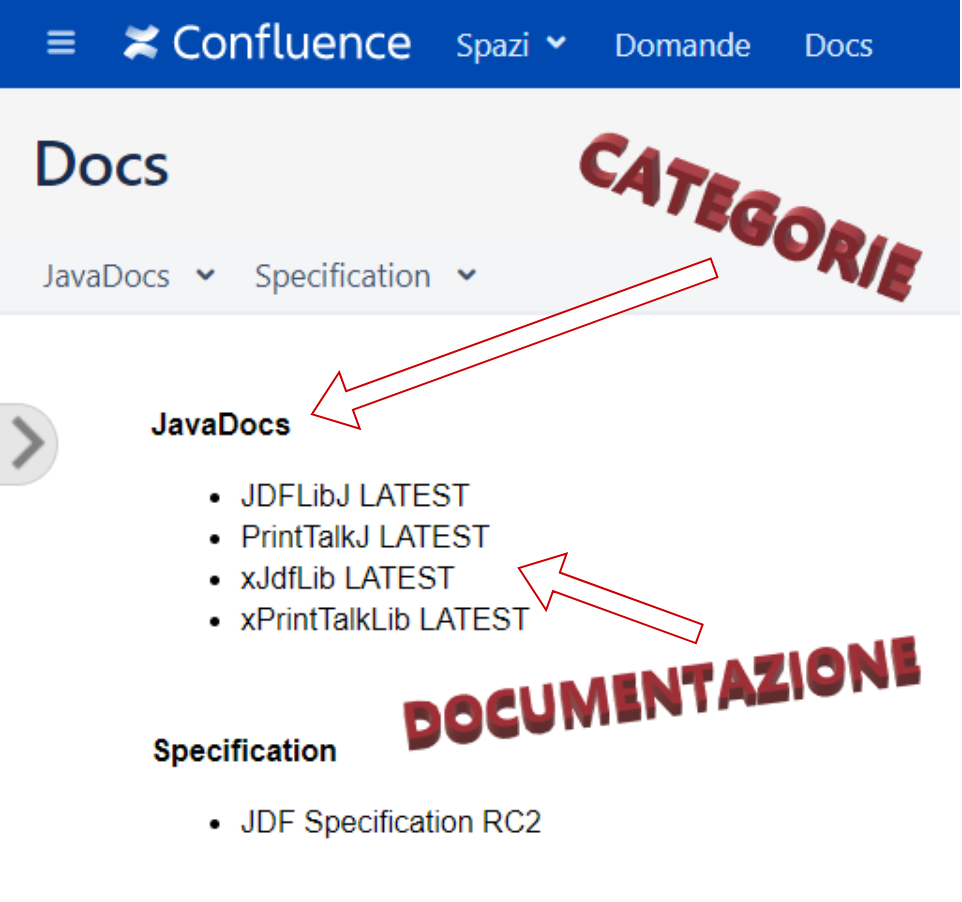
\includegraphics[width=0.7\textwidth]{immagini/docs-conf.png}\\
    \caption{Screenshot di un esempio di Docs Plug-in}
\end{figure}

Ciò che fa il prodotto ottenuto è caricare in maniera automatica la documentazione nella corretta categoria, realizzando un nuovo \emph{doc} o aggiornandone uno esistente.
Nel caso in cui l'utilizzatore del plugin Maven fornisca un titolo per la pagina \emph{doc} che non è presente nel \emph{Docs}, ne verrà creata una nuova, altrimenti il \emph{doc} già esistente con quel nome verrà aggiornato.

%**************************************************************
\section{Organizzazione del testo}

\begin{description}
    \item[{\hyperref[cap:analisi-requisiti]{Il secondo capitolo}}] comprende l'analisi dettagliata dei requisiti del prodotto con casi d'uso e il relativo tracciamento dei requisiti individuati.

    \item[{\hyperref[cap:progettazione]{Il terzo capitolo}}] descrive la progettazione del software.

    \item[{\hyperref[cap:realizzazione-testing]{Il quarto capitolo}}] approfondisce la realizzazione del plugin e come è stata effettuata l'attività di testing.

    \item[{\hyperref[cap:conclusioni]{Il quinto capitolo}}] corrisponde al capitolo conclusivo. Esso riassume il risultato finale ottenuto e attua una valutazine critica del prodotto.

\end{description}

% TODO aggiungere altro
Riguardo la stesura del testo, relativamente al documento sono state adottate le seguenti convenzioni tipografiche:
\begin{itemize}
	% \item gli acronimi, le abbreviazioni e i termini ambigui o di uso non comune menzionati vengono definiti nel glossario, situato alla fine del presente documento;
	% \item per la prima occorrenza dei termini riportati nel glossario viene utilizzata la seguente nomenclatura: \emph{parola}\glsfirstoccur;
	\item i termini in lingua straniera o facenti parti del gergo tecnico sono evidenziati con il carattere \emph{corsivo};
	\item per tutti i concetti che possono essere riassunti, viene fornita una tabella o un elenco puntato.
\end{itemize}